\subsection*{L'analisi dei dati}
\subsection{Moto in discesa}
In questo paragrafo vogliamo analizzare due grafici particolari che sono stati ottenuti da alcuni studenti, come esempio di come può essere condotta l'analisi dei dati di un esperimento.

 Questo è l'aspetto di uno dei grafici:

\begin{figure}[H]
 \centering
 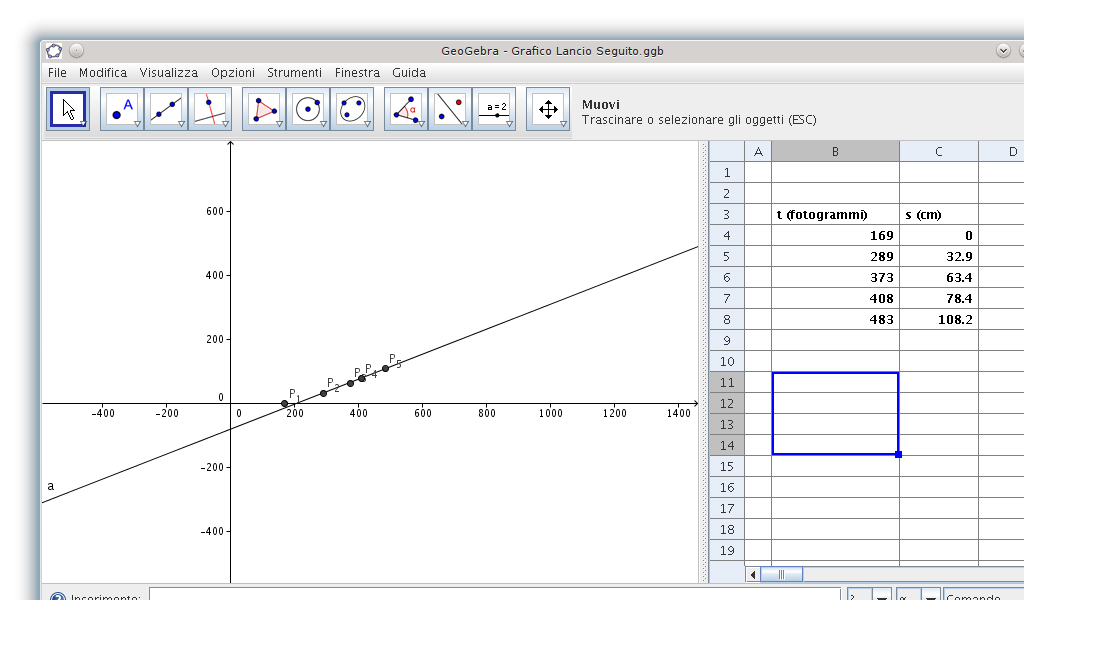
\includegraphics[width=.7\textwidth]{../immagini/discesa.png}
 \label{fig:moto di discesa}
\end{figure}

Come si osserva, quasi tutti i dati sono allineati su una retta ben riconoscibile.\newline
Solo uno dei punti si discosta visibilmente dalla retta.\newline

Per esercizio, valutate le veocità medie per ciscuna coppia di punti sperimentali e valutate se sono tutte uguali tra loro.\newline

La retta tracciata sul grafico non costituisce un rilievo sperimentale, ma una elaborazione realizzata da alcuni studenti sulla base dei dati acquisiti. Per ricavarla, è stato semplicemente estratto un valore credibile per il coefficiente angolare ed imposta la condizione di passaggio per un punto. Un gruppo di studenti più avanzato avrebbe potuto applicare ai dati delle tecniche rigorose di regressione lineare, ma in questo caso, probabilmente, non serve troppa matematica per dare un'intrepretazione fisica accettabile del fenomeno.\newline

Una possibile interpretazione dei dati può essere la seguente:
\begin{center}
\begin{tabular}{||*{3}{p{5cm}|}|}
\hline
Cosa faccio & Cosa osservo & Come spiego \\
\hline
Una pila viene lanciata lungo un piano inclinato con una velocità iniziale modesta. &
La pila accelera per un breve tratto iniziale, ma successivamente si stabilizza in un moto a velocità costante per un tempo piuttosto lungo, che si arresta solamente sulla parete di fondo. &
L'accelerazione iniziale potrebbe far pensare ad una leggera inclinazione del banco, che successivamente scompare o viene equilibrata da qualche altro effetto non facilmente individuabile. \\
\hline
\end{tabular}
\end{center}

\subsection{Moto in salita}
Questo è un secondo grafico:

\begin{figure}[H]
 \centering
 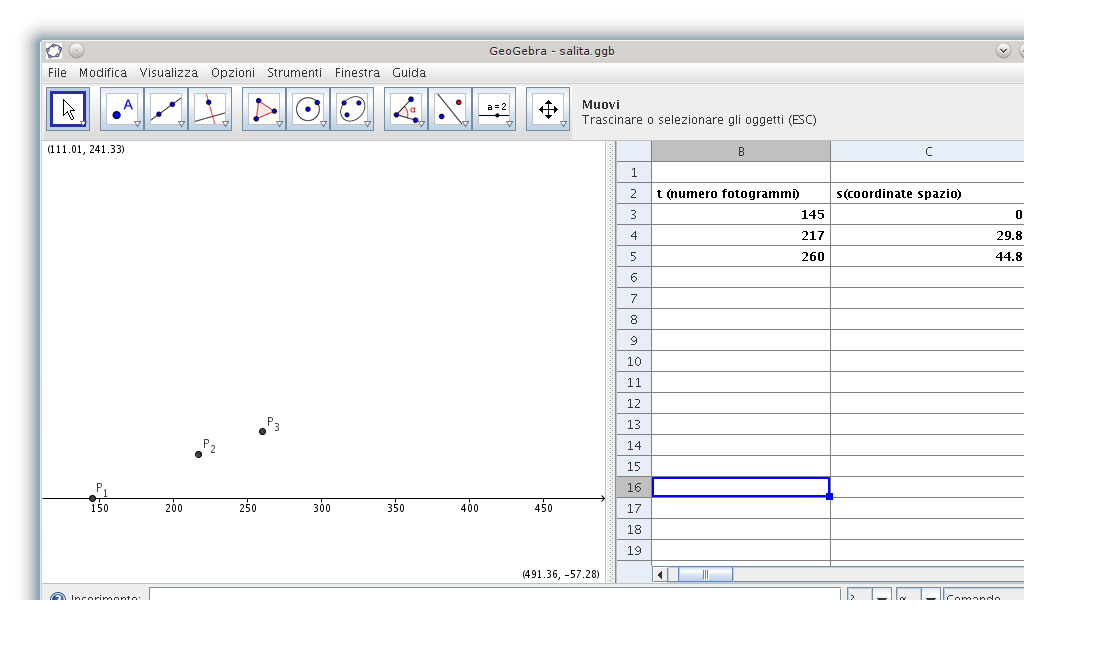
\includegraphics[width=.7\textwidth]{../immagini/salita.png}
 \label{fig:moto di salita}
\end{figure}

È relativo a un lancio della batteria all'indietro. Tutte le volte in cui la batteria è stata lanciata all'indietro, è stata osservata, anche ad occhio nudo, una accelerazione negativa, come se il percorso fosse in leggera salita.

I nostri dati, in questo caso, contengono appena tre punti. Ma questo è il minimo indispensable per distinguere un moto uniforme da uno accelerato.\newline
In effetti il punto $ P_3 $ è troppo basso per essere allineato e il calcolo delle velocità medie indica un rallentamento.\newline

Usando questi tre punti, possiamo valutare l'{\bf accelerazione media} della batteria.\newline
Questo equivale ad assumere che l'equazione del moto corrisponda all'equazione del moto uniformente accelerato:
\begin{center}
  \begin{equation}
  	s = \frac{1}{2} a t^2 + v_0 t + s_0
  \end{equation}
\end{center}

Sostituendo alle variabili $s$ e $t$ le coordinate dei punti $P_1$, $P_2$ e $P_3$, si ottiene un sistema lineare che restituisce i valori dei parametri $a$, $v_0$ e $s_0$.\newline
Volendo, ci si può aiutare con un programma grafico, capace di calcolare l'equazione di una parabola per tre punti e di rappresentarla su un grafico. Qui sotto, mostriamo un'immagine prodotta con kig:

\begin{figure}[H]
 \centering
 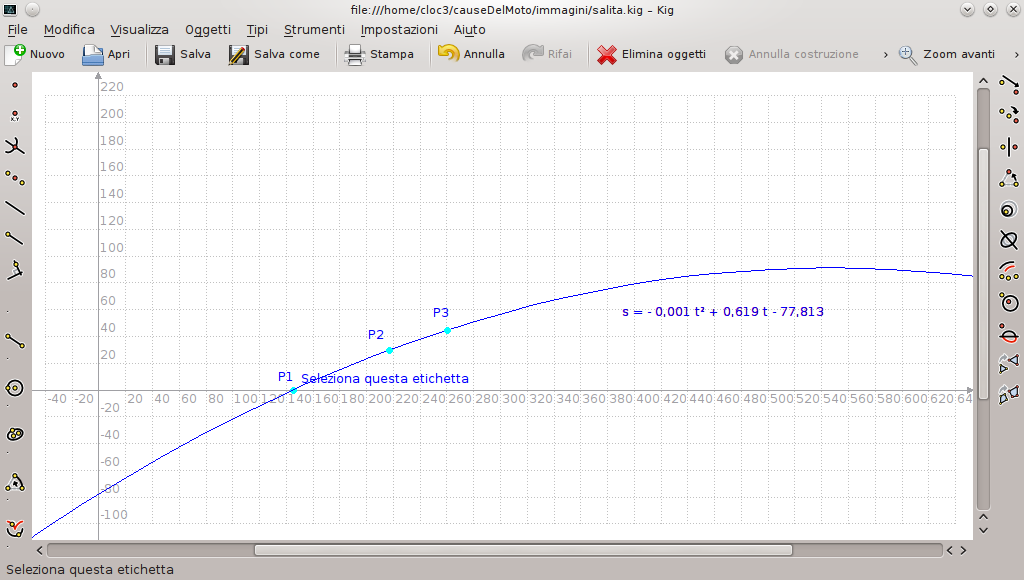
\includegraphics[width=.7\textwidth]{../immagini/salitaConKig.png}
 \label{fig:parabolaPerTrePunti}
\end{figure}

\subsection{Le unità di misura}

Elaborare dei dati non si esaurisce semplicemente nell'uso di programmi grafici che rappresentano i dati acquisiti. È estremamente importante, invece, mantenere il controllo di ciò che i dati significano, cominciando dalla valutazione delle unità di misura. Nel lavoro che stiamo analizzando, i tempi sono determinati dal numero di fotogramma acquisito dalla webcam. L'intervallo di tempo che separa un fotogramma dall'altro è una piccola frazione di secondo.\newline
Le nostre telecamere acquisivano 30 fotogrammi al secondo.\newline

Le lunghezze, invece, sono state acquisite in centimetri. Se desideriamo esprimere le nostre accelerazioni in metri e secondi, dobbiamo considerare che:
\begin{center}
\begin{math}
1 \frac{cm}{{fotogramma}^2}=1 \frac{10^{-2}m}{{(30^{-1}}s)^2} = 9 \frac{m}{s^{-2}}
\end{math}
\end{center}

Osserviamo anche che il programma kig produce una stima dell'accelerazione con una sola cifra significativa, che è riduttiva per la precisione con la quale abbiamo raccolto i notri dati. Questa sezione, relativa alla elaborazione dei dati, può quindi assumere gradi diversi di approfondimento, che sono lasciati alla determinazione dell'insegnante.
